\documentclass[bsc,frontabs,twoside,singlespacing,parskip]{infthesis}

\title{Data Gathering Performance and Spatial Prediction for Mobile Air Quality Monitoring}
\author{Dale Myers}
\date{April 3, 2014}
\course{Master of Informatics}
\project{{\bf MInf Project (Part 2) Report}}


\usepackage{tabularx}
\usepackage{float}
\usepackage{url}
\usepackage{verbatim}
\usepackage{fixltx2e}
\usepackage{parskip}
\usepackage{hyperref}
\usepackage{minted}
\usepackage{upgreek}
\usepackage{comment}
\usepackage{pdflscape}
\usepackage{amsmath}
\usepackage{footnote}
\usepackage{longtable}
\usepackage{subcaption}
\usepackage{afterpage}
\usepackage[demo]{graphicx}
\usepackage[version=3]{mhchem}
\usepackage[colorinlistoftodos,textwidth=2.0cm]{todonotes}
\usepackage[toc,page]{appendix}
\usepackage{caption}
\usepackage{titlesec}

\let\oldtodo\todo
\newcommand{\maheshi}[1]{\oldtodo[inline,color=green!40]{#1}}
\newcommand{\mahesh}[1]{\oldtodo[color=green!40, size=\tiny]{#1}}
\newcommand{\idea}[1]{\oldtodo[inline,color=blue!40]{#1}}
\newcommand{\tdi}[1]{\oldtodo[inline]{#1}}
\renewcommand\todo[1]{\oldtodo[size=\tiny]{#1}}


\newcommand{\todohidden}[1]{}

\newcommand{\tdic}[2][]{
    \oldtodo[inline, caption={#1}]{
        \begin{minipage}{
            \textwidth-4pt
        }
        #2
        \end{minipage}
    }
}

\newcommand{\plan}[2][]{
    \oldtodo[inline, caption={#1},color=blue!40]{
        \begin{minipage}{
            \textwidth-4pt
        }
        #2
        \end{minipage}
    }
}


\newcommand{\code}[2]{
    \inputminted[mathescape,linenos,numbersep=5pt,frame=lines,framesep=2mm]{#1}{#2}
}

\newcommand{\centerimagewideanywhere}[3]{
    \begin{figure}[h]
        \begin{center}
            \includegraphics[width=\textwidth]{#1}
            \caption{#2}
            \label{#3}
        \end{center}
    \end{figure}
}

\newcommand{\centerimagewide}[3]{
    \begin{figure}[H]
        \begin{center}
            \includegraphics[width=\textwidth]{#1}
            \caption{#2}
            \label{#3}
        \end{center}
    \end{figure}
}

\newcommand{\centerimageanywhere}[4]{
    \begin{figure}[h]
        \begin{center}
            \includegraphics[width=#1]{#2}
            \caption{#3}
            \label{#4}
        \end{center}
    \end{figure}
}

\newcommand{\centerimage}[4]{
    \begin{figure}[H]
        \begin{center}
            \includegraphics[width=#1]{#2}
            \caption{#3}
            \label{#4}
        \end{center}
    \end{figure}
}

%Temporary fixes for todonotes
\hbadness=10000
\vbadness=10000
\setlength{\marginparwidth}{2cm}


\setcounter{secnumdepth}{4}
\setcounter{tocdepth}{4}


\begin{document}

\pagenumbering{gobble} %This suppresses an error with the hyperref package

%Abstract based on the one from: http://homepages.inf.ed.ac.uk/mmarina/papers/ipin13b.pdf
\abstract{
Air quality measurements in urban environments are on the rise. In this study we look at the performance of using Lothian Buses as a mobility mechanism for air quality sensors in the city of Edinburgh. Specifically, through the means of simulation, we evaluate the various parameters of such a model, discovering that using opportunistic forwarding provides the greatest benefit to such a system. We then use data similar to that generated by such a system to evaluate the effectiveness of various simple spatial interpolation methods on urban air quality data sets. We find that natural neighbour interpolation gives the best performance, but not with accuracy great enough to be used for any formal scientific context.
}

\maketitle
\newpage

\section*{Acknowledgements}

First and foremost I would like to thank my supervisor Dr Mahesh Marina for all the time and effort he put into helping me mould and form this project and report. His thoughtful input and personal experience helped drive this project forward. 

I would also like to thank Professor D K Arvind, Dr Stratis Viglas and Dr Paul Patras for their help and experience with simulating networked environments. 

For their help with data collection, I would like to thank Dr Jane Hillston, the staff at Lothian Buses, and all members of the OpenSense group. 

Finally, I would like to thank my family and friends for all their support and encouragement over the course of this project. 

%Mahesh
%DK and Stratis for simulator
%Paul Patras for help with Omnet++
%Jane and Lothian buses for the bus data
%

\tableofcontents
\newpage

\listoftodos
\newpage

%\listoffigures
%\tdi{This will be removed}
%\newpage

%\listoftables
%\tdi{This will be removed}
%\newpage

\pagenumbering{arabic}


\chapter{Introduction}\label{introduction}

    Hurr
    \tdi{Have a motivation behind the work}
    \tdic[Project Goals]{Indicate the goals of the project in crisp terms (simulation is a means)
        \begin{itemize}
            \item Study the data gathering performance in a bus based monitoring system for air quality
            \item Methodology\: Simulation
            \begin{itemize}
                \item Evaluate and optimise
            \end{itemize}
        \end{itemize}
    }
    \tdi{Accomplishments in terms of addressing those goals}
    \tdi{This is how the rest of the report looks}

\chapter{Background and Related Work}\label{background}




\section{Previous Work}\label{background_previous_work}

    %Talk about everything. Even the stuff I didn't use
    %The AP data from Arsham

    In the first year of this project much of the initial research was done. In this section some of the key topics will be briefly discussed.

    \subsection{Air Quality}\label{background_air_quality}

A definition of air quality is a difficult problem which has not been solved. Many institutions measure and record what they refer to as ``air quality'', however the only thing these measurements have in common is that no two are the same. In order to research the area of ``air quality'' further we must have a concrete definition of what air quality is. Current definitions give a simple definition of ``air quality'' as being antonymous to that of air pollution in that higher air quality is the equivalent to low air pollution~\cite{bcaq}. This implies that not only should the metrics used for defining air quality be considered, but also those used to define air pollution.

Looking at statements and measurements by various authorities around the world \cite{epapollutants,airqualityobjectives,cleanairnavigation,naaqs,whoguidelines}, we can build a list of common pollutants which are measured:


\begin{itemize}
\item Sulphur dioxide
\item Nitrogen dioxide
\item PM10 
\item PM2.5
\end{itemize}

These chemicals can form the basis of pollutants which in turn can help define ``air quality''. By looking at other sources~\cite{meaningsofenvironmentalterms},  proposed definition of ``air quality'' is as follows:

\begin{quote}
``The current measurements of the concentrations of certain pollutants in the air relative to the requirements of one or more biotic species or to any human need or purpose.''
\end{quote}


    \subsection{Geostatistical Mapping}
    
        It was discovered that when working with an actual data set, obtained by using a sensor built by a previous years student, \emph{Eric Staples}, work would have to be performed in order to make use of the data effectively. Generally, heat maps are used to show various concentrations and levels of variables in a two dimensional environment and so the same would be used in this project. The interpolation method which should be used was a more difficult problem. Initial research suggested that some form of convolution filter, or blur, when applied to a sufficiently dense data set would give a reasonable approximation, however this was later found to be incorrect, and would not apply to a sparse data set likely to be generated from any experiments. Further research showed that when interpolating environmental data such as pollutant levels, the most common method is kriging, a statistical method which fits a curve to the data set. Kriging is used as the basis for many advanced models~\cite{regressionkriging}.

    \subsection{Compressive Sampling}

        Compressive sampling was looked into briefly as a method of enhancing our data collection methodology. The basis behind compressive sampling is that more measurements are taken in areas of high variance, with less measurements taken in areas of lower variance~\cite{compressivesampling}. Essentially this is a variable method of conforming to the Nyquist theorem, which is discussed further in section~\ref{prediction_evaluation_motivation}. The work on this area was discovered to involve much background research into the nature of the pollutants and the areas they build up and would not work if there were a change to this environment. As such this technique was not used in the final solution.

    \subsection{Sensor Creation}

        Initially this project was intended to have a practical component, however external circumstances restricted this and the physical implementation was cancelled. Before this change, research was done into building a physical sensor using cheap, off the shelf parts, which would be dynamically calibrated using the techniques discussed in the D. Hasenfratz et al. paper titled ``On-the-fly calibration of low cost gas sensors''\cite{ontheflycalibration}. Individual sensors were researched and purchased in order to make a prototype, before the physical implementation was cancelled. 
    

\section{Interpolation Methods}\label{background_interpolation_methods}
    This section focuses on the various statistical methods of interpolating and extrapolating data values at arbitrary points on a grid. These methods vary in their effectiveness on different data sets, however it is important to note that none of these methods take into account data which could be viewed as extremely important in this case. An example of this is the terrain. In section \todo{Fill in this reference} we discuss the effect that canyoning has on air quality readings. This effect is ignored by these models. 

    A further crucial piece of information which needs to be taken into account is that these models do not take into account temporal changes of readings. In order to use our data sets we will have to have a way of ``snapshotting'' data. A choice needs to be made for the length of time each snapshot should be. A suggestion for a rough value is 30 minutes, however experimental results will reveal the best value to use.

    With regards to the models chosen, various possibilities were considered. Due to the fact that various algorithms are similar with minor differences, the decision was made to use only a single algorithm from each ``family''. As such the algorithms chosen to be evaluated are:

    %http://en.wikipedia.org/wiki/Multivariate_interpolation
    \begin{itemize}
        \item Bicubic interpolation
        \item Natural neighbour interpolation
        \item Spline interpolation
        \item Nearest neighbour interpolation
        \item Inverse distance weighting interpolation
        \item Barnes interpolation
    \end{itemize}

    These algorithms can be split into two categories, regular grid algorithms and irregular grid algorithms, based on the format of the input data expected. 

    \subsection{Regular Grid Algorithms}\label{background_interpolation_methods_regulargrid}

        These interpolation methods require a regular grid with data points placed onto them and will calculate all missing values. In order to conform to this the data into ``buckets''. Buckets of around $5m^{2}$ will allow us to have a reasonable resolution for data without our calculations taking too long. The boxed area which the trams cover in Zurich is roughly $5km^{2}$. This gives us a grid resolution of 1,000*1,000, for a total of 800,000 data points. 

        \subsubsection{Bicubic}\label{background_interpolation_methods_bicubic}

            Bicubic interpolation is the simplest of the grid interpolation algorithms which will be evaluated. As a cubic Hermite spline~\cite{practicalguidesplines} the output is smoother than linear interpolation methods such as bilinear interpolation, as we can see in figure~\ref{fig:bicubicvsbilinear}. The bicubic algorithm achieves this by taking into account the 16 points surrounding the point to be interpolated rather than just 4. 

            \centerimage{\textwidth}{images/Bicubic_vs_Bilinear_Interpolation.png}{This figure, created by Wikipedia user \emph{Berland}, shows the difference between bicubic interpolation (left) and bilinear interpolation (right) on the same dataset.}{fig:bicubicvsbilinear}\mahesh{Should this be in italics?}

            The algorithm for bicubic interpolation is relatively simple, with the result being given by the calculation:

            \begin{align*}
                p(x,y) = \sum_{i=0}^{3}{\sum_{j=0}^{3}{a_{ij}x^{i}y^{j}}}
            \end{align*}

        %\subsubsection{B\'{e}zier Surface}\label{background_interpolation_methods_beziersurface}
        %Probably not since the surface is stretched towards the points, but does not pass through them
        
        %\subsubsection{Lanczos Resampling}\label{background_interpolation_methods_lanczosresampling}
        %Used to interpolate between a sampled signal.
        
        %\subsubsection{Delaunay Triangulation}\label{background_interpolation_methods_delaunaytriangulation}
        %Doesn't give a smooth curve


        \subsubsection{Barnes}\label{background_interpolation_methods_barnes}

            Barnes interpolation uses a multi-pass approach to determine the new data points. The method has found success in calculating air pressure across the United States, providing results similar to careful analysis, however it depends on the data points be reasonably uniform~\cite{barnesinterpolation}.

            No examples existed in either R or Python and so a custom implementation written in Python was created. This implementation follows the information in the original paper by Barnes and has shown success on test data sets. The algorithm works by calculating a simple distance weighted interpolation as the first result, and then iterating multiple times using a calculated error field to reduce the errors in the output. 

            One important factor in Barnes interpolation is the fact that it depends on server constants. These constants depend on the type of data being interpolated and the nature of the measurements, including the density of the measurements. As such, determining these constants is a key part of using this algorithm for interpolation. One advantage of this approach, is that we can iterate over our data set and fit it to the known measurements in order to make sure it is as accurate as possible. With this method however, we lose test data points and so cannot validate it. Experiments using this algorithm have used similar mechanisms and shown success~\cite{pmconcentrationmaps}.

            The algorithm for Barnes interpolation is as follows.

            For the first pass each known point is assigned a weight using the formula: 

            \begin{align*}
                W_{i} &= e^{-(d/R^{2})}
            \end{align*}
            
            where d is the distance between the known point and the current point to be interpolated, and R is the radius of influence. Using this weight, the initial guess of the grid points is calculated as: 
            
            \begin{align*}
                X_{g} &= \frac{\sum_{i}{W_{i}X_{i}}}{\sum_{i}{W_{i}}}
            \end{align*}

            At this point we begin our successive passes. These are defined as:

            \begin{align*}
                X'_{g} &= X_{g} + \frac{\sum_{i}{W'_{i}E_{i}}}{\sum_{i}{W'_{i}}}
            \end{align*}

            where $E_{k}$ is the difference between the estimated value and the actual value at a known point $k$ and $W'_{i}$ is defined as:

            \begin{align*}
                W'_{i} &= e^{-(d/\Gamma R)^{2}}
            \end{align*}

            with $\Gamma$ as a convergence parameter normally set in the range 0.2-0.3.

            The created Python code for this algorithm is as follows:

            \tdi{Fix this code and make it nice.}
            \inputminted[mathescape,linenos,numbersep=5pt,frame=lines,framesep=2mm]{python}{../Data/OpenSense/barnes.py}

        
        \subsubsection{Natural Neighbor}\label{background_interpolation_methods_naturalneighbour}
        %Seems like an interesting successor to bicubic
        
        \subsubsection{Spline Interpolation}\label{background_interpolation_methods_splineinterpolation}
        %Basic spline method

    \subsection{Irregular Grid Algorithms}\label{background_interpolation_methods_irregular_grid}

        %\subsubsection{Radial Basis Function}\label{background_interpolation_methods_radial_basis_function}
        %The value will dip between points so probably not what is needed

        %\subsubsection{Thin Plate Spline}\label{background_interpolation_methods_thin_plate_spline}
        %Seems complicated

        %\subsubsection{Least-Squares Spline}\label{background_interpolation_methods_least_squares_spline}
        %A possibility

        %http://en.wikipedia.org/wiki/Nearest-neighbor_interpolation
        \subsubsection{Nearest Neighbour}\label{background_interpolation_methods_nearest_neighbour}

            Nearest neighbour interpolation is the simplest interpolation we will see in that it is not really interpolation at all. Instead the value of each point is the value of the closest data point we have. A na\"{\i}ve version of the algorithm in Python, with \emph{known\_points} being a list of tuples containing the co-ordinates and value of each known point, is as follows\:

            \inputminted[mathescape,linenos,numbersep=5pt,frame=lines,framesep=2mm]{python}{../Data/OpenSense/nearest_neighbour.py}

        \subsubsection{Inverse Distance Weighting}\label{background_interpolation_methods_inversedistanceweighting}

            Inverse Distance Weighting, known as IDW, is the second simplest algorithm. Each point is a weighted average of all known points, where the weighting is the inverse of the distance. 

            Each value is calculated as follows:

            \begin{align*}
                V = \frac{\sum_{i=1}^{n}{\frac{v_{i}}{d^{p}_{i}}}}{\sum_{i=1}^{n}{\frac{1}{d^{p}_{i}}}}
            \end{align*}

            Once again, there are parameters which must be supplied to the algorithm which are data dependent. In this case the parameter is the smoothing factor. A lower smoothing factor means that the interpolated value at a known data point is closer to the value of the known data point. A higher smoothing factor makes the rate of change smaller to give a smoother graph and the cost of some interpolated points being different to known values which are nearby.

        %\subsubsection{Kriging}\label{background_interpolation_methods_kriging}
        % Very complicated and requires a lot of domain specific knowledge


\section{Mobile Sensing Models}\label{background_mobile_sensing_models}

\maheshi{Not sure about this section at all. In terms of mobile sensing models I could talk about some of the different experiments that have been done such as CarTel, Cafnet and OpenSense, but I would only be touching upon this again, and stating what they do?}


\section{Wireless Propagation Models}

    \maheshi{Not sure how much to write about this? It is a complex area and if I go into it any further I'd spend the remaining two weeks just reading up on this.}

    When implementing a simulation of wireless communications one of the decisions which must be made is which radio propagation model to use. These propagation models define how different signals behave under different conditions and are generally given in terms of a mathematical equation. Using these models we can enter information about our radio signal, such as frequency, transmitter power and receiver power,  and gain information such as the signal to noise ratio of the signal over some distance.

    In Omnet++, which is the simulator we end up using, there are six different models implemented. These models are ``Free Space Model'', ``Two Ray Ground Model'', ``Rice Model'', ``Rayleigh Model'', ``Nakagami Model'' and ``Log Normal Shadowing Model''. The Free Space model is the simplest of these models and acts the same way a signal would in ``free space''. That is to say, a space where there is no interference from external signals, or the original signal through reflection, refraction or diffraction. This model is usually used as a component of other models and formulae~\cite{friis1946note}.

    The two ray ground model is only slightly more advanced, in that it takes into account a singular reflection from some boundary, usually the ground~\cite{tworaygroundmodel}.

    The log normal shadowing model builds on this. This model has two variable parameters, $\gamma$ and $\sigma$, which are used to tune the model to the environment. Other formulations have up to 5 parameters. These parameters provide information about the types of obstacles they are likely to experience and are generally provided through empirical analysis~\cite{goldhirsh1998handbook}.

    Nakagami's distribution is a variation of a gamma distribution in that we provide two parameters to this model, $m$ and $\Omega$, which control the shape of the distribution. In order to achieve a propagation model, this distribution is applied to the power level~\cite{nakagamipowerlevel}.

    The Rice model, also known as the Longley-Rice model, has origins in telecommunications. Originally designed to take into account the terrain, it can require up to 11 input parameters~\cite{ricemodel}. This model is complicated, but provides accurate information, and indeed is used by the US Federal Communications Commission~\cite{fcclongleyrice}.

    The final model is the Rayleigh model. This model works by assuming that fading happens according to a random distribution when passing through some material. This model has shown promising results in dense urban environments~\cite{rayleighmanhattan}.




\chapter{Simulation Environment}\label{simulation}

    \tdi{Mention that all I had to do was add the mobility in essence.}
    
    One of the main goals of this project is to study the performance of an urban mobile air quality monitoring system leveraging public transport vehicles, including the effects of various parameters including number of roadside access points, storage capacity (queue size) on mobile sensor platforms. Due to various reasons, working with actual buses proved to be impossible. As such the decision was made to make simulation the mechanism through which the performance of this model would be evaluated. 

    We wish to model buses moving around the city of Edinburgh with air quality sensors attached. These buses would communicate with open IEEE 802.11 wireless access points as they move around the city, uploading the data they recorded to a central server. In order to model these buses as accurately as possible we required data about existing buses. Initially the attempt was made to use the Lothian Buses API, which can be seen in action at the website: \href{http://www.mybustracker.co.uk/}{\nolinkurl{http://www.mybustracker.co.uk/}}. However, due to the lack of position information this approach was quickly discarded. Talks with Lothian Buses gave access to 24 hours worth of position data of their ``liveried'' fleet. These are the buses which have route specific colouring and graphics. In total we have access to 145 different buses with position data for each bus with a maximum of 30 seconds between position readings. In order to simplify the work with the simulator, where the movement steps happen every second, the data was interpolated using a simple linear interpolation algorithm to a 1 second resolution. We chose a resolution of 1 second for movement as we can approximate the movement between data points without doing extra calculations with little benefit. The interpolation can cause some deviation from the correct path around corners, however, due to the fact that buses in Edinburgh can travel no faster than 30mph, which is approximately 13.4m/s, the buses can travel at most 402m between readings. This will only happen should the bus be travelling in a straight line at this constant maximum speed. By adding in a corner, which is where we would see deviation from the actual path, we can be at most 142m, proven via trigonometry, from the true position. The chances of this happening are extremely low however and it is likely that we will be much closer. This error, while potentially lowering the efficiency of our algorithm slightly, is unlikely to have a large effect.

    With regards to the data for the wireless points, this data was provided by Ph.D. student Arsham Farshad, who travelled around Edinburgh on various buses, recording the locations of wireless access points, and more importantly, those which are open. From the initial choice of roughly 2000 access points, the 82 with the strongest signal, when measured from a bus, were chosen. As will be seen in section~\ref{simulation_simulator_options_simulation_speed_optimisation}, the processing time of the simulation is heavily dependent on the number of access points. Due to this no simulation is run with more than 50 access points. 

    \section{Simulator Options}\label{simulation_simulator_options}

        In simulating a complex model like this, certain questions need to be answered and challenges overcome. This section answers these questions, such as ``what simulator should be used?'', and ``how can we use it as efficiently as possible?''. 

        \subsection{Simulator Choice}\label{simulation_simulator_options_simulator_choice}

            The initial simulator choice of \emph{NS-3} was recommend by Dr. Marina. NS-3 was recommended due to its reputation for being extremely powerful and realistic. This reputation has caused NS-3 to be used in various projects and experiments with great success~\cite{highperformancesimulatorofadhocnetworks}.  Further more, when compared with other well known network simulators, such as NS-2, Omnet++ and JiST, it performed the best overall~\cite{networksimulatorcomparison}. NS-3 was created as the successor to the older simulator NS-2. The main changes between versions was changing from using a scripting language to create simulations in a dedicated application, to becoming a framework which can be embedded in any application, with support for both C++ and Python. 

            Initial simulation tests were completed with NS-3, however after almost 4 weeks of testing it became clear that the learning curve of NS-3 was significant, and was in danger of delaying the progress of the entire project. Due to this danger other simulators were explored. 

            Omnet++ (\emph{Objective Modular Network Testbed in C++}) was the suggestion of Dr. Arvind and Dr. Viglas who have supervised students using this simulator. Research into the simulator showed that Omnet++ is not a network simulator in the same way that NS-3 is. Instead, it is a framework which uses discrete events as its basis. Simulations for Omnet++ are also written in C++, but follow a different approach. The simulator uses a collection of modules which follows a strict object oriented model. New modules can be created by sub-classing others, or simply connecting them together into a greater module. With respect to these modules, there are many different collections of these modules, known as ``models''. Many models exist for Omnet++ including, but not limited to, Castilla, INET and MiXiM, with the latter two being of particular interest. In terms of performance and accuracy, Omnet++ rivals NS-3~\cite{networksimulatorcomparison}.

            MiXiM is used in Omnet++ for creating wireless networks with a particular focus on the lower layers of the network stack. The models provided in the MiXiM framework are extremely detailed and include radio wave propagation, interference estimation, radio transceiver power consumption and wireless MAC protocols~\cite{miximvision}. MiXiM has no support for the upper network layers and if you need these then you need to rely on another model such as INET, or create your own. The features in MiXiM are extremely advanced and it was therefore decided that it is more complex than required for this application. While it wouldn't change the results by using MiXiM, it would slow the simulation down considerably.

            INET is very closely related to Omnet++ in that it is rare to use Omnet++ without using INET. INET provides models for the internet stack, as well as wired and wireless link layer protocols. It also contains many different application layer models, mainly for demonstration purposes.  


        \subsection{Data Collection}\label{simulation_simulator_options_data_collection}

            \tdi{Wondering if this is worth even mentioning? It did form a significant part of the project.}

            One of the further advantages of choosing Omnet++ was that it had a rather sophisticated data logging framework built in. This framework made it extremely easy to record information about the simulations, such as packet loss, latency and throughput. It was soon discovered however that this came at a price. After running a simple simulation with all 145 buses and 50 access points for a simulated time of 10,000 seconds, the output of this logging frame work was measured at over 40GB. Further more, it was not in an easily accessible format for further analysis using a scripting language. As such, the decision was made to create a logging framework which would reduce the size of these data files. Running the same simulation with the new framework reduced the file size to around 3GB, which when compressed came down to around 200MB. This huge space saving allowed for more simulations to be run as the data did not have to be collected at the end of each simulation to avoid running out of disk space. 

        \subsection{Simulation Speed Optimisation}\label{simulation_simulator_options_simulation_speed_optimisation}

            When the simulation was completed, multiple tests were run in order to profile the performance of the simulator and simulations. The results of this profile can be seen in figure~\ref{fig:access_points_vs_time_and_events}. These results show that when there are no buses, the number of simulation events per second increases with the number of access points. The relationship is polynomial in nature, but only to a small degree. The reasoning for this being that most access points are not in range of any others when we have a lower number of them and so they do not have any effect on each other. The number of events is correlated with the simulation time. That is, the more events there are per second, the longer it will take to simulate one second of time. 

            When we add in our buses we can see that things change dramatically. The number of events now increases exponentially with the number of access points. This has a similar effect on the total simulation time, causing it to also increase exponentially. 

            Due to these effects, we cannot feasibly run simulations with more than 50 access points. According to figure~\ref{fig:access_points_vs_time_and_events}, increasing to just 60 access points would almost double our total simulation time. 

            \centerimagewideanywhere{./images/AP_vs_Time_and_Events.png}{An example of how simulation time and events change with the number of access points.}{fig:access_points_vs_time_and_events}\todo{Replace with matplotlib version}

            When running a full simulation with 50 access points and all 145 buses it took around 3 days to simulate just 1 day. In order to be able to perform all desired experiments and be able to repeat them multiple times in the 6 months which remained at this point, the simulation would have to be improved dramatically. Fortunately Omnet++ provided a mechanism for this. 

            \emph{MPI}, which stands for Message Passing Interface, is supported by Omnet++~\ref{omnetmpi}. MPI allows simulations to run on multiple cores concurrently. Ordinarily Omnet++ runs on a single core, however if it were to use MPI on a 4 core machine then theoretically it is possible to achieve speed boosts of up to 4 times faster. In practise it is lower due to the message passing overhead, but we would still hope to see the simulation time half. The simulation configuration was configured to allow MPI and some speed tests were run. The results of these tests showed that the simulation was almost twice as slow when using MPI. Further investigation revealed the cause of these problems. 

            
            \tdi{Insert figure of bipartite network}

            MPI in Omnet++ works extremely well when the networks are cleanly partitioned. For instance, modelling two subnets connected by a switch. Figure~\ref{????} shows a logical point to partition the network. In this example, one subnet would run on one core, and the other on a separate core. All communication within the subnet would remain on that core, which would cause no additional overhead. Any communications between subnets would then use MPI. In our model we do not have any clean point to partition. With 145 buses moving all over the city and 50 access points it would be difficult to devise an optimal partition. This problem could be solved using machine learning, however it is beyond the scope of this project. It is theorised that if all entities, that is the buses and access points, were run on a separate core, perhaps using many machines, we may see a performance boost, however this was infeasible. 

            Due to parallelising a single simulation failing, a different approach was taken. Instead of running one simulation on $n$ cores, the decision was made to run $n$ simulations on $n$ cores, essentially one simulation per core. Initial testing was performed on a dual core machine with two simulations. The results showed that the simulations both took more than twice as long as the single test. When this was tested on a quad core machine however, the simulations took slightly less than double the time. This means that the total time to run both simulations was less than running each sequentially, which is a clear improvement. Unfortunately continuous access to this quad core machine was not available and an alternative had to be found. 

            Currently, popular methods of performing large scale computations are to use virtual machines hosted by a third party. \todo{Think this paragraph needs reworded.} Common companies to use for this are \emph{Amazon}, \emph{Rackspace} and \emph{Digital Ocean}. Based on the requirements above, the aim would be to choose multiple instances with 4 cores for the cheapest price. In terms of cost, Digital Ocean was a clear winner, however it was 4 times as expensive to get a 4 core machine as it was to get a 2 core machine. As such, simulations were run on 5 dual core machines. Each machine was given a different random sampling of access points, and all simulations on each machine were run sequentially. This reduced the run time of some test from over a month to just under a week. 


    \section{Opportunistic Forwarding}\label{simulation_opportunistic_forwarding}

        \tdi{I don't mention packet latency at all.}
        \tdi{Talk about 125 buses instead.}

        Air quality has been measured using vehicles before such as with the OpenSense project, however these project tend to rely on cellular connectivity for returning the data. Our system does not use cellular connectivity and instead relies on open wifi access points. This method presents certain problems. The main problem being that we have no control over the location of these access points and as such buses may spend a long time out of range of an access point, or indeed may not even come into contact with one at all. Figure~\ref{fig:access_point_map} shows the locations of the 82 access points in Edinburgh we will be using for our simulations. We can see that these access points are clustered around the centre of the city and there are almost none at all at distances of more than 2 miles from the centre. 

        \centerimagewideanywhere{./images/APMap.png}{A map of all 82 open access points which are used in our simulations.}{fig:access_point_map}

        From this image we can see that it is likely that we will run into issues should there be any buses which do not go through the city centre as part of their route. Unfortunately this is the case for a particular route. Buses on route 39 do not travel inside the city bypass at all, a boundary which is generally regarded as the bounds of the city. These buses travel around some of the villages in the south of the city. There are no access points outside the bypass. Route 39 is shown in figure~\ref{fig:route_39}.

        \centerimagewideanywhere{./images/Route39.png}{Lothian bus route 39.}{fig:access_point_map}

        Based on the chemicals discuss in section~\ref{background_air_quality}, we know how much data we need to store for each data packet. The total size of each packet is 24 bytes and the composition of each packet is laid out in table~\ref{tab:data_packet}. Research in the first year of this project into creating a physical sensor revealed that the \emph{Arduino Uno} would make a good choice of base component. The reasons for this included it's cost, size, and use in similar projects~\cite{arduinoproj1}~\cite{arduinoproj2}~\cite{arduinoproj3}. The Uno's main problem however is the limited space for storing data. The standard version has just 32,256 bytes of storage space available~\cite{arduinounospecs}. This means that it can store at most 1,344 packets. With a new measurement every second this amounts to just over 22 minutes of data storage space. A more expensive version has storage space for 10,581 packets, which is just under 3 hours of recording. Ideally we would need at least one full days worth of storage space to ensure that all the recorded data makes it back to the central server since the buses return to a depot within the city at night should they not be in use. In order to ensure that we don't end up with only the last 22 minutes of data for the buses on route 39, and indeed the last 22 minutes before finding an access point on routes which only have minimal access to access points, we need a different method of returning the data.

        \begin{table}
            \centering
            \begin{tabular}{ | c | c |}
                \hline
                Metric & Size (bytes)\\ \hline
                Timestamp & 4 \\
                Bus Id & 2 \\
                \cee{CO_{2}} & 2 \\
                \cee{NO_{x}} & 2 \\
                \cee{O_{3}} & 2 \\
                PM 10 & 2 \\
                PM 2.5 & 2 \\
                Latitude & 4 \\
                Longitude & 4 \\
                \hline
                Total & 24 \\
                \hline
            \end{tabular}
            \caption{The layout of a single data packet.}
            \label{tab:data_packet}
        \end{table}

        The solution for this is known as \emph{opportunistic forwarding}. Opportunistic forwarding consists of buses communicating with one another and passing the data between them so that as much data as possible will be returned to the central server with the lowest possible latency. An example of how this works can be shown using the buses on route 39. On this route there is a straight which the buses on route 40 also traverse. The buses on route 40 however travel into the city and come into contact with access points. This can be seen in figure~\ref{fig:route_39_40}. When a bus on route 39 comes into contact with a bus on route 40, the buses exchange information about who will find an access point the soonest and the space they have available. In this case the bus on route 40 will come into contact with an access point first and so will accept the data from the route 39 bus. The bus on route 40 will accept as many packets as it can without causing it to lose any of its own between now and finding an access point. This is achieved by each bus being able to predict when it will come into contact with an access point. In reality this would be achieved by programming this buses with timetables and recording data about the access points they met. We can simulate this past data by giving it the actual location data which has been slightly ``fuzzed''\todo{No. Just no.} in order to make it more representative of what we would actually be working with. 

        \centerimagewideanywhere{./images/Route3940.png}{Lothian bus routes 39 and 40.}{fig:route_39_40}

        In order to simulate opportunistic forwarding certain decisions had to be made. \todo{Do I say this too much?} The first decision to be made is how the opportunistic forwarding will be realised. In a physical implementation, the standard mechanism would be to use a single radio and switch back and forth between the peer to peer communication mode and the access point detection mode. The reason for doing this is purely cost based. With a simulator we are not limited to this and as such we add a second radio. The addition of a second radio would add a fraction of a second delay to connecting to an access point when we come across one (when we do find one we will stop trying to send data to other buses), which is a penalty worth taking for the simplification of the model. 

        The more important decision to be made is the algorithm we will use in our model. Lebrun et al. discussed five different algorithms for opportunistic forwarding~\cite{opportunisticforwarding}. These algorithms were \emph{NOTALK}, \emph{BROADCAST}, \emph{Location-based}, \emph{MoVe} and \emph{MOVE-Lookahead}. NOTALK is the base case in which there is no communication between nodes and so will be discounted immediately. BROADCAST is the opposite in that every sensor exchanges information with every other sensor it comes into contact with. This method of routing is known as \emph{epidemic routing}, and was first described by Vahdat et al. in \emph{Epidemic routing for partially connected ad hoc networks}~\cite{vahdat2000epidemic}. The goals and therefore advantages of epidemic routing, and therefore broadcast BROADCAST, as described in the Vahdat et al. paper are ``i) maximize message delivery rate, ii) minimize message latency, and iii) minimize the total resources consumed in message delivery.'' Using opportunistic forwarding removes one of the main requirements of other routing algorithms which is the assumption that a path to an access point always exists. The price we pay for these advantages however is the large storage space requirements. Obviously this limitation is one which cannot be ignored due to the reasons discussed above and as such we need to discount the BROADCAST algorithm. The MoVe and the MOVE-Lookahead algorithms require much more information than we have available and must be discounted. This leaves us with one algorithm and that is the Location-based algorithm. This algorithm is derived from the BROADCAST algorithm by employing a heuristic. The heuristic is that the algorithm only passes on the data to the other sensor should it reach an access point first. This is the algorithm which was implemented. 

        The algorithm employs the following approach for the broadcasting bus, A:


        \begin{enumerate}
            \item Broadcast first packet in queue to all nearby buses
            \item If we receive a response, remove the packet from our queue and repeat
            \item If we do not receive a response then try again in 0.5 seconds
        \end{enumerate}

        For the receiving bus, B:

        \begin{enumerate}
            \item Compare the time until bus A will reach an access point (AP) to the time that this bus, B, will reach an access point using the information in the packet.
            \item If bus A reaches an AP first then discard this packet and do not respond.
            \item If bus B will reach an AP first then predict how much ``spare'' space bus B will have in it's buffer when reaching the AP:
                \begin{enumerate}
                    \item Calculate time until next AP, $t$.
                    \item Subtract $t$ from space remaining, $r$, and call this result $s$.
                \end{enumerate}
            \item If $s$ is greater than 0 then accept this packet by adding it to our own queue and broadcasting a response.
        \end{enumerate}

        In order to successfully use this algorithm we need to provide extra information in our packets we send. This extra information includes the time until finding the next access point (4 bytes) and the identifier of the bus the packed \emph{originated} from (2 bytes). This addition of 6 bytes changes our packet size to 30 bytes in total. Which means that each device can no longer hold 1,344 packets and instead can only hold 1,075 packets, or in the case of the larger storage space it changes from 10,581 to 8,465. This is 18 minutes and 141 minutes of data respectively. As will be shown in chapter~\ref{data_gathering_performance} the trade off is justified. 


\chapter{Data Gathering Performance}\label{data_gathering_performance} 

    \todo{This title needs to reflect the first goal of the project}

    The first and foremost goal of this project is to study the performance of an urban mobile air quality monitoring system which leverages public transport vehicles and the effects of various parameters. In order to do this we must decide on how we will measure the performance as well as what parameters we will vary. 

    In order to measure the performance of the system, we must pay attention to the use of such a system. With air quality sensors on buses our priorities are receiving as much data as possible and receiving said data with minimal latency. These priorities define our metrics for us. Our metrics shall be the percentage of readings which are returned to the server, and the time which it takes for this to happen. In doing this we must consider how the effects of varying different parameters change the results. The parameters which we will vary are the storage space on the device, that is to say how many packets we can store in the queue at any one time, the number of access points scattered around the city, the power levels of the transmitter and receiver and finally the utility of using a priority queue instead of a regular queue when using opportunistic forwarding.
	

    \section{Queue Size}\label{data_gathering_performance_queue_size}

        \tdi{Reword the end of this.}

        Varying the size of the queue was a simple change but one which would yield great insight. The queue size is how many packets or readings we can store on the sensor at any one time. When creating a physical implementation of this model one of the prohibiting factors is cost, and the storage size is almost directly correlated with the cost of the device. As such it is extremely important to evaluate the effectiveness of the model when using a smaller queue size. In order to test this, we ran the simulation with all 145 buses and 50 access points but a variable queue size. The sizes of queue checked were 10, 30, 100 and 2000. The results of running this simulation, a can be seen in table~\ref{tab:queue_size} and figure~\ref{fig:queue_size}. 

        From the data it is clear that having a larger queue size has a positive effect on the percentage of packets which are delivered. In fact, we can see that we more than triple the packet delivery rate by increasing the queue size from 10 packets to 2000. Tripling the queue size from 10 until 30 has a relatively small performance increase. Due to this, it is theorised that even if the queue were non existent we would not decrement our percentage of packets received by a significant amount. The reason for this is that 14\% is likely to be close to the mean amount of time that a bus is in contact with an access point for. When a bus is in contact with an access point it can send the packets immediately without losing them. With a buffer size of 10, we can only store packets for 10 seconds before contacting an access point. If the mean amount of time a bus is in contact with an access point is 10 seconds, then removing this queue size would halve the packet delivery rate. From this we can see that the smaller the queue size, the less effect it has on the packet delivery percentage. However, following the trend from this information, it would require a queue size of between 150,000 and 200,000 in order to get a 100\% packet delivery rate. In terms of storage space this is between 3.6MB and 4.8MB. However, 150,000 readings is just under 42 hours worth of data. We can expect an upload of at least every 24 hours or 86,400 seconds and so there is no need for the size to be greater than this, nor can we trust the results. 

        As the queue size increases we increase the ratio of packets delivered but also increase the latency. This is an expected behaviour due to the fact that more packets will be stored and therefore they have an effect on the latency. 

        \begin{landscape}
            \begin{table}
                \centering
                \begin{tabularx}{\linewidth}{|X|X|X|X|X|X|X|X|}
                    \hline
                    \multicolumn{1}{|X|}{\centering Queue \\ Size} & 
                    \multicolumn{1}{|X|}{\centering Number \\ of APs} & 
                    \multicolumn{1}{|X|}{\centering Mean \\ Latency (s)} & 
                    \multicolumn{1}{|X|}{\centering Standard \\ Deviation (s)} & 
                    \multicolumn{1}{|X|}{\centering Packets \\ Sent} & 
                    \multicolumn{1}{|X|}{\centering Packets \\ Received} & 
                    \multicolumn{1}{|X|}{\centering Packets \\ Dropped} & 
                    \multicolumn{1}{|X|}{\centering \% \\ Received} \\
                    \hline
                    10 & 50 & 0.485136283 & 0.482648346 & 2726636.5 & 207879.1667 & 1049162.833 & 14.34 \\
                    30 & 50 & 3.075895053 & 3.067765 & 2757366.667 & 238289.5 & 1020537.167 & 16.43 \\
                    100 & 50 & 16.72300115 & 16.72759292 & 2826758 & 307587.5 & 955076.8333 & 21.21 \\
                    2000 & 50 & 419.8375185 & 420.5738133 & 3220432.833 & 700218.1667 & 537348.1667 & 48.29 \\
                    \hline
                \end{tabularx}
                \caption{The results of changing the number of access points.}
                \label{tab:num_aps}
            \end{table}
        \end{landscape}

        \tdi{Insert chart of this data here}

    \section{Number of Access Points}\label{data_gathering_performance_number_of_access_points}

        The interest in varying the number of access points (APs) stems from the fact that this is a variable which is outwith our control. By setting a performance target we can find the minimum number of access points we would need to meet this target. This will show us if our system could potentially work in a situation with less APs (in reality there are many more). The results of varying the number of APs under different queue sizes is shown in table~\ref{tab:num_aps} and figure~\ref{fig:num_aps}.

        \begin{landscape}
            \begin{table}
                \centering
                \begin{tabularx}{\linewidth}{|X|X|X|X|X|X|X|X|}
                    \hline
                    \multicolumn{1}{|X|}{\centering Queue \\ Size} & 
                    \multicolumn{1}{|X|}{\centering Number \\ of APs} & 
                    \multicolumn{1}{|X|}{\centering Mean \\ Latency (s)} & 
                    \multicolumn{1}{|X|}{\centering Standard \\ Deviation (s)} & 
                    \multicolumn{1}{|X|}{\centering Packets \\ Sent} & 
                    \multicolumn{1}{|X|}{\centering Packets \\ Received} & 
                    \multicolumn{1}{|X|}{\centering Packets \\ Dropped} & 
                    \multicolumn{1}{|X|}{\centering \% \\ Received} \\
                    \hline
                    10 & 10 & 0.641546601 & 0.628416482 & 2837154.833 & 77350 & 1166151.5 & 5.33 \\
                    10 & 20 & 0.6377266 & 0.629448882 & 2806916.5 & 116009.5 & 1132689.333 & 8.00 \\
                    10 & 30 & 0.591328457 & 0.581260675 & 2775618.5 & 153667.3333 & 1098895.167 & 10.60 \\
                    10 & 40 & 0.557965006 & 0.552124348 & 2754254.5 & 179980.5 & 1076107.833 & 12.41 \\
                    10 & 50 & 0.485136283 & 0.482648346 & 2726636.5 & 207879.1667 & 1049162.833 & 14.34 \\
                    30 & 10 & 4.016328768 & 3.955641293 & 2851801 & 91969.33333 & 1151698.333 & 6.34 \\
                    30 & 20 & 3.978558616 & 3.946152299 & 2829299.333 & 138289.1667 & 1111176 & 9.54 \\
                    30 & 30 & 3.70040839 & 3.653918235 & 2802597.667 & 180843 & 1072978 & 12.47 \\
                    30 & 40 & 3.468226904 & 3.445352797 & 2783234.5 & 209719.8333 & 1047929 & 14.46 \\
                    30 & 50 & 3.075895053 & 3.067765 & 2757366.667 & 238289.5 & 1020537.167 & 16.43 \\
                    100 & 10 & 25.04383636 & 24.87469435 & 2898691.5 & 138808.1667 & 1105236.667 & 9.57 \\
                    100 & 20 & 23.43013378 & 23.36990619 & 2893541.833 & 202327.5 & 1049191 & 13.95 \\
                    100 & 30 & 20.75840795 & 20.63997577 & 2872975.833 & 250772.3333 & 1005479.667 & 17.29 \\
                    100 & 40 & 19.17159602 & 19.16736037 & 2856199.833 & 282431.8333 & 978600.3333 & 19.48 \\
                    100 & 50 & 16.72300115 & 16.72759292 & 2826758 & 307587.5 & 955076.8333 & 21.21 \\
                    2000 & 10 & 617.8010824 & 617.0399697 & 3369388.667 & 608908.8333 & 614393.3333 & 41.99 \\
                    2000 & 20 & 518.9917672 & 519.4679392 & 3351993.5 & 660129.8333 & 570220.6667 & 45.53 \\
                    2000 & 30 & 468.1774747 & 468.9056058 & 3302144.333 & 679437.8333 & 554234.8333 & 46.86 \\
                    2000 & 40 & 436.3411623 & 436.5999819 & 3271823.667 & 697031.5 & 539818.6667 & 48.07 \\
                    2000 & 50 & 419.8375185 & 420.5738133 & 3220432.833 & 700218.1667 & 537348.1667 & 48.29 \\
                    \hline
                \end{tabularx}
                \caption{The results of changing the number of access points.}
                \label{tab:num_aps}
            \end{table}
        \end{landscape}

        \tdi{Insert chart of this}

        From this data we can see that the greater the number of access points the lower the latency and the greater the packet delivery rate. When adding a larger queue size the packet delivery rate increases but there is no improvement in latency, which manifests as a latency increase overall. With increasing the number of APs that disadvantage is no longer present. At smaller queue sizes we can double or even triple the packet delivery rate with more access points. It should be noted that as discussed in chapter~\ref{simulation} simulation time was one of the main factors for limiting the simulations to at most 50 access points. With the dataset we had over 2,000 access points. As such we can expect a much greater packet delivery rate with a significantly lower mean latency in an actual realisation of this model. 


    \section{Transmitter and Receiver Power}\label{data_gathering_performance_transmitter_and_reciever_power}

        A simple way of increasing the access point coverage of the city is to increase the power levels of the access points and receivers. This increase in power level causes them to serve a greater area without the need for any more access points. European legislation restricts all 2.4GHz radios to an equivalent isotropically radiated power level of 100mW~\cite{rackley2011wireless}. Converting to dBm gives a value of 19.93dBm, or approximately 20dBm. In practice we cannot increase the power levels of the radios without breaking the law, however we can do this with a simulator. In order to determine the effect that power level has on the data collection performance we tested the model at 5 different power levels. These power levels were 18, 19, 20, 21 and 22 dBm, which corresponds to 64.00, 80.63, 101.59, 128.00 and 161.27 respectively. Furthermore, we also must acknowledge that this is in fact a simulation and therefore not identical to a physical implementation. As such we need to also acknowledge that the propagation model will not be perfect. In order to find the most realistic model for our simulation we tried using 2 different models for this test. These propagation models were the Rayleigh model and the Log Normal Shadowing model. The results of this test, using a queue size of 2000 and all 50 access points, are shown in table~\ref{tab:power_level} and figure~\ref{fig:power_level}. 

        \begin{landscape}
            \begin{table}
                \centering
                \begin{tabularx}{\linewidth}{|X|X|X|X|X|X|X|X|X|}
                    \hline
                    \multicolumn{1}{|X|}{\centering Power} & 
                    \multicolumn{1}{|X|}{\centering Model} & 
                    \multicolumn{1}{|X|}{\centering Mean \\ Latency (s)} & 
                    \multicolumn{1}{|X|}{\centering Standard \\ Deviation (s)} & 
                    \multicolumn{1}{|X|}{\centering Packets \\ Generated} & 
                    \multicolumn{1}{|X|}{\centering Packets \\ Sent} & 
                    \multicolumn{1}{|X|}{\centering Packets \\ Received} & 
                    \multicolumn{1}{|X|}{\centering Packets \\ Dropped} & 
                    \multicolumn{1}{|X|}{\centering \% \\ Received} \\
                    \hline
                    18 & Rayleigh & 154.12 & 323.82 & 294,743.60 & 522,092.80 & 238,455.20 & 1,986.40 & 80.74 \\
                    18 & Log Normal Shadowing & 122.62 & 278.35 & 279,041.50 & 452,601.00 & 225,997.50 & 2,268.75 & 79.72 \\
                    19 & Rayleigh & 128.94 & 281.37 & 270,759.00 & 473,615.20 & 213,552.20 & 933.20 & 78.72 \\
                    19 & Log Normal Shadowing & 169.79 & 363.87 & 527,232.75 & 868,566.75 & 431,838.25 & 34,279.50 & 83.15 \\
                    20 & Rayleigh & 150.13 & 322.72 & 299,218.50 & 525,681.25 & 240,421.75 & 1,445.50 & 80.26 \\
                    20 & Log Normal Shadowing & 150.72 & 316.18 & 470,629.50 & 782,219.50 & 388,500.00 & 20,491.00 & 81.03 \\
                    21 & Rayleigh & 116.22 & 255.51 & 220,911.00 & 383,434.50 & 169,469.00 & 0.00 & 76.79 \\
                    21 & Log Normal Shadowing & 86.43 & 203.14 & 179,300.00 & 290,371.00 & 134,968.00 & 0.00 & 75.27 \\
                    22 & Rayleigh & 135.75 & 294.37 & 270,957.00 & 471,525.67 & 218,749.33 & 977.33 & 80.54 \\
                    22 & Log Normal Shadowing & 0 & 0 & 0 & 0 & 0 & 0 & 0 \\
                    \hline
                \end{tabularx}
                \caption{The results of changing the power level of the radios.}
                \label{tab:power_level}
            \end{table}
        \end{landscape}

        In terms of the propagation model a significant problem was found which may be apparent from the final row in table~\ref{tab:power_level}. There appeared to be a bug in the implementation in Omnet++ in which the simulation tended to crash when used with this simulation after some indeterminable period of time. Generally we did not get a simulation time of longer than 2,000 seconds which is significantly shorter than the 10,000 seconds we had been using previously. In some cases we did not get readings for particular runs using the Log Normal Shadowing model and therefore the mean result was made up of just 3 or 4 readings instead of 5. Furthermore, the effect that the software bugs had on the simulation when also trying the Log Normal Shadowing model also seemed to affect the simulation when going using the Rayleigh model, which is the model used for all other experiments. As such no further experiments were performed on propagation models. 

        With the results we have we can still analyse the effect that power level has. The effect is almost non-existent. We would expect to see a decrease in latency and increase in packet delivery as the power level goes up, however we saw no such increase. It is theorised that the reason for this is that the packet upload time is dominated by the bandwidth of the connection. By increasing the power levels we may be in contact with an access point for an extra few seconds, however as we can upload 2000 packets in less than a second, which is an effective rate of 48Kbps, this extra time only limits the delivery time of a single packet or two. Over a greater period of time, should the simulation have not crashed, it is possible that we may have seen a very small correlation, however it is insignificant at this time. 


    \section{Opportunistic Forwarding}\label{data_gathering_performance_opportunistic_forwarding}

        Opportunistic forwarding is the most significant change to the model that we will attempt. The implementation details are discussed in section~\ref{simulation_opportunistic_forwarding}. With the implementation discussed, the only way to evaluate the performance is to run a simulation both with and without opportunistic forwarding. The results of this are shown in table~\ref{tab:opportunistic_forwarding} and figure~\ref{fig:opportunistic_forwarding}.

        \begin{landscape}
            \begin{table}
                \centering
                \begin{tabularx}{\linewidth}{|X|X|X|X|X|X|X|X|X|X|X|}
                    \hline
                    \multicolumn{1}{|X|}{\centering Queue Size} & \multicolumn{1}{|X|}{\centering Mean Latency (s)} & \multicolumn{1}{|X|}{\centering Standard Deviation} & \multicolumn{1}{|X|}{\centering AP Received} & \multicolumn{1}{|X|}{\centering AP Unique} & \multicolumn{1}{|X|}{\centering Packets Sent} & \multicolumn{1}{|X|}{\centering Packets Successful} & \multicolumn{1}{|X|}{\centering Packets Stored} & \multicolumn{1}{|X|}{\centering Packets Dropped} \\
                    \hline
                    10 & 0.23 & 1.39 & 463,908 & 421,622 & 2,160,545 & 463,239 & 57,673 & 833,967 \\
                    30 & 1.52 & 5.96 & 626,482 & 499,921 & 2,200,064 & 598,384 & 128,859 & 759,144 \\
                    100 & 12.02 & 30.38 & 829,123 & 513,153 & 2,490,028 & 733,816 & 341,718 & 753,631 \\
                    1000 & 236.26 & 370.09 & 1,475,528 & 659,686 & 4,063,488 & 1,121,781 & 1,827,617 & 438,549 \\
                    2000 & 344.52 & 633.09 & 1,534,024 & 648,545 & 4,825,887 & 1,109,934 & 2,605,998 & 289,271 \\
                    \hline
                \end{tabularx}
            \end{table}
            \begin{table}
                \centering
                \begin{tabularx}{\linewidth}{|X|X|X|X|X|X|X|X|X|X|X|}
                    \hline
                    \multicolumn{1}{|X|}{\centering Queue Size} & \multicolumn{1}{|X|}{\centering AP Received} & \multicolumn{1}{|X|}{\centering AP Unique} & \multicolumn{1}{|X|}{\centering Packets Sent} & \multicolumn{1}{|X|}{\centering Packets Successful} & \multicolumn{1}{|X|}{\centering Packets Stored} & \multicolumn{1}{|X|}{\centering Packets Dropped} & \multicolumn{1}{|X|}{\centering Queue Ignores Time} & \multicolumn{1}{|X|}{\centering Queue Ignores Space} & \multicolumn{1}{|X|}{\centering Queue Ignores Ratio} & \multicolumn{1}{|X|}{\centering \% Received} \\
                    \hline
                    10 & 463,908 & 421,623 & 2,160,545 & 463,239 & 57,673 & 833,967 & 8,183,045 & 8,567,042 & 0.955 & 33.73\% \\
                    30 & 626,482 & 499,921 & 2,200,064 & 598,384 & 128,859 & 759,144 & 7,126,313 & 7,348,423 & 0.975 & 39.99\% \\
                    100 & 829,123 & 513,153 & 2,490,028 & 733,816 & 341,718 & 753,631 & 8,189,153 & 8,429,989 & 0.971 & 41.05\% \\
                    1000 & 1,475,528 & 659,686 & 4,063,488 & 1,121,781 & 1,827,617 & 438,549 & 6,906,153 & 6,976,392 & 0.990 & 52.77\% \\
                    2000 & 1,534,025 & 648,545 & 4,825,887 & 1,109,934 & 2,605,998 & 289,271 & 5,808,998 & 5,644,930 & 1.030 & 51.88\% \\
                    \hline
                \end{tabularx}
            \end{table}
        \end{landscape}


    \section{Priority Queue}\label{data_gathering_performance_priority_queue}

        \plan[Priority Queue]{Explain how queue size changed things}
        %Only 125 buses

    \section{Conclusions}\label{data_gathering_performance_conclusions}

        \plan[Conclusions]{Conclude with summary}
        %Remember that this is just 145 buses

\chapter{Prediction Evaluation}\label{prediction_evaluation}
	
	
	\tdic[Prediction is inevitable]{Intro talks about no matter how we do it the data will be spatially incomplete. Prediction is inevitable
		\begin{itemize}
			\item Explain different ones here (can link to background section). Are they any use? Can simple things work?
			\item Extra stuff is beyond the scope of this work
		\end{itemize}
	}
	\tdi{Explain how I will study the performance of the data set}
	\tdi{Present and discuss results}


	Stampfenbachstrasse: (47.386769, 8.539810)
	Schimmelstrasse: (47.370962, 8.523560)

	The remaining part of the project is evaluating whether the implementation would provide useful data or not. As mentioned in section ??\todo{Fill in this reference} a similar project is currently running in Zurich. The \emph{OpenSense}~\cite{opensensezurich} project places sensors on trams and is designed to provide data to the general public with minimal cost. The project uses cheap hardware and accurate stationary measurement stations for calibration. If we look at their maps of information we can see that the readings they provide are only along the tram routes. An example of this, but in Edinburgh, can be seen in figure~\ref{fig:stationarypollutantbuildup}. In order for the data that we would potentially collect, should the project be physically realised, to be useful we would have to be able to accurately predict what the concentrations of chemicals are in areas where we do not have sensor readings. 

	\begin{figure}[H]
	    \begin{center}
	        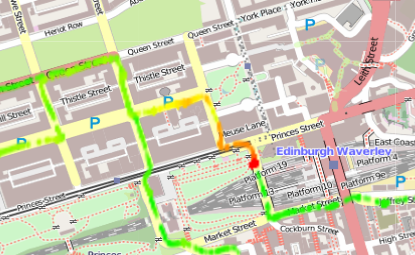
\includegraphics[width=\textwidth]{./images/StationaryPollutantBuildUp.png}
	        \caption{A map of air pollution around Edinburgh city centre. Image uses \emph{Open Street Map}.}
	        \label{fig:stationarypollutantbuildup}
	    \end{center}
	\end{figure}

	If were were to use some statistical method on a dataset similar to that seen in figure~\ref{fig:stationarypollutantbuildup}, we could estimate with some degree of certainty what the pollution levels are in areas where there are no recordings. By doing this we could produce a map similar to the one in figure~\ref{fig:zurichheatmap}.

	\begin{figure}[H]
	    \begin{center}
	        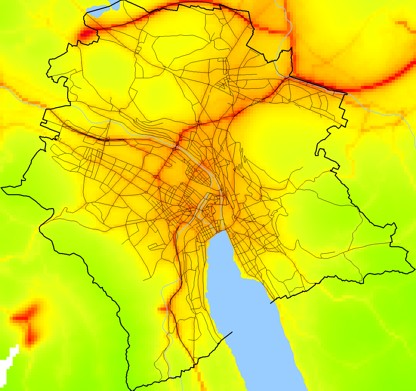
\includegraphics[width=\textwidth]{./images/zurichpm.jpg}
	        \caption{A heatmap of particulate matter in Zurich. The higher pollution levels can clearly be seen to follow transport infrastructure.~\cite{opensensezurich}}
	        \label{fig:zurichheatmap}
	    \end{center}
	\end{figure}

	
	In order to solve this problem and accurately predict the pollution levels, advanced statistical techniques, with a great deal of domain specific information, are required. Doing this would be impractical for the \emph{City of Edinburgh Council}. Instead we will employ existing tools and simpler statistical methods to help us perform this task. By using well known and understood methods, avoiding complex methods such as regression kriging~\cite{regressionkriging}, which are provided in a single tool or package, such as R or Python libraries, we will attempt to prove that this data is at least accurate enough to provide a high level overview of pollution across the city. 

	In order to validate whether our results are correct or not, we will use the freely available data from the OpenSense project and perform our analysis on this. By performing our statistical methods on a dataset from the OpenSense project we will be able to predict the pollution levels at any point in Zurich to within some degree of accuracy. By comparing the values at the same locations as a static measurement station, with the results from said measurement station, we will obtain a metric which informs us of the accuracy of the interpolation method.



\chapter{Conclusions}\label{conclusions}


The main goals of this project were to evaluate the performance of using public transport as the mechanism for mobile air quality monitoring systems, and to evaluate the effectiveness of using common spatial prediction methods to interpolate the results from such a system. This report looked at how to simulate such a model, methods of evaluating the performance of the model, and various interpolation methods for interpolation the data. In terms of evaluating the performance metric we learned some key pieces of information. 

The first and foremost of these is that using the Lothian Bus services in Edinburgh, connecting to IEEE 802.11 access points, provides around 50\% of the total readings using a queue size which would be suitable in commodity hardware which would be used to build such a sensor. The mean time between these readings being taken and being returned to a central server is approximately seven minutes. This is within acceptable ranges for most applications, however we would hope to have a latency of under a minute for ``real-time'' applications. In terms of air quality measurements there is no definition of ``real-time'' however it is difficult to imagine applications which would require a smaller delay as minor fluctuations in measurements would distort the data so much that interpretation would be difficult. The results from varying parameters with this algorithm are consistent with what we would expect to see in that having more access points causes the packet delivery rate to go up and the latency to go down. We also showed that increasing the queue size increased the rate of packets being delivered, while also increasing the latency as more packets are stored for longer. 

Adding opportunistic forwarding was an extremely successful approach. The effect of opportunistic forwarding was much greater at smaller queue sizes than at larger queue sizes. We improved the results over the non-opportunistic method by a factor of 2.6 and 1.4 at queue sizes of 10 and 2,000 respectively. These results were an approximate boost of 20\% of the total number of packets. With regards to the algorithm it was discovered that emulating the non-opportunistic model with the queues, by inserting received broadcast packets at the correct location based on measurement time, was in fact detrimental to the performance of the model. The performance of the model was improved by simply appending the received broadcast packets to the end of the queue. Finally we learned that with opportunistic forwarding we require many fewer access points in order to achieve the same performance as the non-opportunistic model. This requirement implies that we can use this mechanism in smaller cities or towns effectively. 

The simulation was not without flaw however and the results we have are only relative performance metrics. The most important problem with this model was the inability to model all access points within the city. Despite having information about all access points in the city of Edinburgh which are discoverable on buses and open to public access, we were only able to simulate at most 50 of these before the simulation time was too long to realistically consider. The results however show in all cases that increasing the number of access points has a positive effect in terms of packet delivery rates and latency reduction. Due to this we can surmise that in practice this model would achieve better results than are shown in this report. 

In terms of boosting the results one of the implications we must consider is that we have data for 145 buses. Lothian Buses have a fleet of over 700 buses~\cite{lothianbusannualreport} and it is potentially the case, however unlikely, that all buses could be equipped with air quality sensors. Increasing the number of buses has an indeterminable effect currently, however it is hypothesised that the increase in the number of buses would increase the number of successful packet deliveries while also reducing the latency, with the potential for packet duplication eventually becoming an issue and detrimental to the results. This area requires further study. An alternative is using the same number of buses, or indeed fewer buses, but changing which buses are used. Currently the buses are limited to just 13 different routes. By changing the buses which we attach sensors to we can increase the area which our measurements cover. Lothian Buses currently offer 70 different routes which would give us a wide area of coverage. However, by having different routes, it is less likely that our buses will encounter each other as they move and as such the opportunistic forwarding may produce inferior results. Further research into this area is still required.

Looking to our evaluation of simple interpolation algorithms for generating continuous data sets we discovered that reasonable results are generated, however these would be unsuitable for any scientific purpose. We found that when comparing similar algorithms, the ones which have variable parameters tended to produce better results as they are trained to the nature of the data. 


In summary, it has been shown that using Lothian Buses as the mechanism for mobile air quality measurements, uploading to IEEE 802.11 access points, with opportunistic forwarding would be a successful endeavour. The packet delivery rate is relatively high with a reasonable latency period. Using simple interpolation algorithms to gain more useful information was less successful, however we have seen that we can get reasonable results to some degree of certainty which is useful for a more broad overview, but of less use for more advanced applications. As discussed in the background section, there are existing models which generate useful results from such data sets and as such these should be used in practice. 



%\bibliographystyle{unsrt}
\bibliographystyle{plain}
\bibliography{references}

\appendix
\chapter{Appendix}\label{Appendix}

    \section{Code Samples}
        
        \subsection{Barnes Interpolation Algorithm}

            \tdi{Fix this code and make it nice, including comments}
            \code{python}{../Data/OpenSense/barnes.py}

        \subsection{Nearest Neighbour Interpolation Algorithm}

            \code{python}{../Data/OpenSense/nearest_neighbour.py}

        \subsection{Inverse Distance Weighting Interpolation Algorithm}

            \code{python}{../Data/OpenSense/idw.py}

        \subsection{Bicubic Interpolation Algorithm}

            \code{python}{../Data/OpenSense/bicubic.py}

        \tdi{Add bilinear and natural neighbour}



\end{document}



